\documentclass[11pt]{article}
\usepackage[czech]{babel}                                                       
\usepackage[colorinlistoftodos]{todonotes}                                      
\usepackage{comment}                                                            
\usepackage[hidelinks,unicode]{hyperref}                                        
\usepackage{alltt}                                                              
\usepackage[a4paper,left=1.8cm,right=1.8cm,top=1.8cm,textheight=25.0cm]{geometry}
\usepackage[T1]{fontenc}                                                        
\usepackage[utf8]{inputenc}                                                     
\usepackage{xcolor}    
\usepackage{graphicx}


\usepackage{lipsum}

\newcommand\blfootnote[1]{%
  \begingroup
  \renewcommand\thefootnote{}\footnote{#1}%
  \addtocounter{footnote}{-1}%
  \endgroup
}

\begin{titlepage}                                                               
    \title{Databázové systémy \\ Dokumentace projektu}                              
    \author{
        Ondřej Keprt \quad \href{mailto:xkeprt03@stud.fit.vutbr.cz}{xkeprt03@stud.fit.vutbr.cz}\\
        Vladimír Drengubiak \quad \href{mailto:xdreng01@stud.fit.vutbr.cz}{xdreng01@stud.fit.vutbr.cz}
    }                                                                       
\end{titlepage}                                                                 
                                                                                 
\setlength{\marginparwidth}{2cm} %warning handler

\begin{document}
    \maketitle

\section{Zadání}
Rozhodli jsme se pokračovat v zadání projektu z předmětu IUS: 58. Fitness centrum

Navrhněte jednoduchý IS fitness centra, které organizuje různé kurzy skupinových lekcí
(zumba, TRX, kruhový trénink, atd.). Ve fitness centru pracují instruktoři, kteří vedou 
jednotlivé skupinové lekce, a lidé na recepci, kteří se musí kromě vítání příchozích klientů
a mixování proteinových koktejlů zapojit do práce s IS fitness centra prostřednictvím
vytváření členských karet pro jednotlivé klienty, kteří se rozhodli pravidelně trápit svá těla 
ve fitness centru a chtějí využít členské výhody. Aby karta nebyla využívána jinými klienty 
než jejím vlastníkem, musí být v IS uloženy základní informace o klientech, jejich rodná čísla 
a adresy. Zákazník si může vypsat kurzy, které navštěvuje a informace o jednotlivých lekcích. 
Navíc si může zobrazit rozvrh vypisovaných kurzů a zjistit počet volných míst na jednotlivých 
lekcích a jejich cenu. Zákazník se může registrovat buď na jednu lekci nebo na celý kurz. 
Kurzy mají svou délku trvání, obtížnost a popis. Skupinové lekce probíhají v různých sálech 
fitness centra, které mají konkrétní název, umístění a maximální kapacitu. Lekce jsou vedené 
jedním instruktorem, mají maximální kapacitu účastníků a odehrávají se v daném sále v určitý 
čas a den v týdnu. Předpokládejte, že jeden instruktor může být vyškolen pro vedení různých 
kurzů, toto modelujte. Kromě pravidelných skupinových lekcí nabízí fitness centrum i 
individuální lekce, na kterých se instruktor věnuje pouze jednomu klientovi. Tyto lekce jsou 
podobného charakteru jako ty skupinové, jen je konkrétnímu klientovi věnováno více pozornosti. 
Instruktor má možnost vložit do systému nové typy kurzů a konkrétní lekce (a to jak skupinové, 
tak i individuální) a měnit čas a sál, ve kterém se lekce konají. Systém musí být na požádání 
schopen vypsat rozvrh pro jednotlivé místnosti.

\newgeometry{left = 0cm,right = 0cm}
\begin{figure}[ht]
    \caption{Schéma databáze generované pomocí SQL Developeru}    
    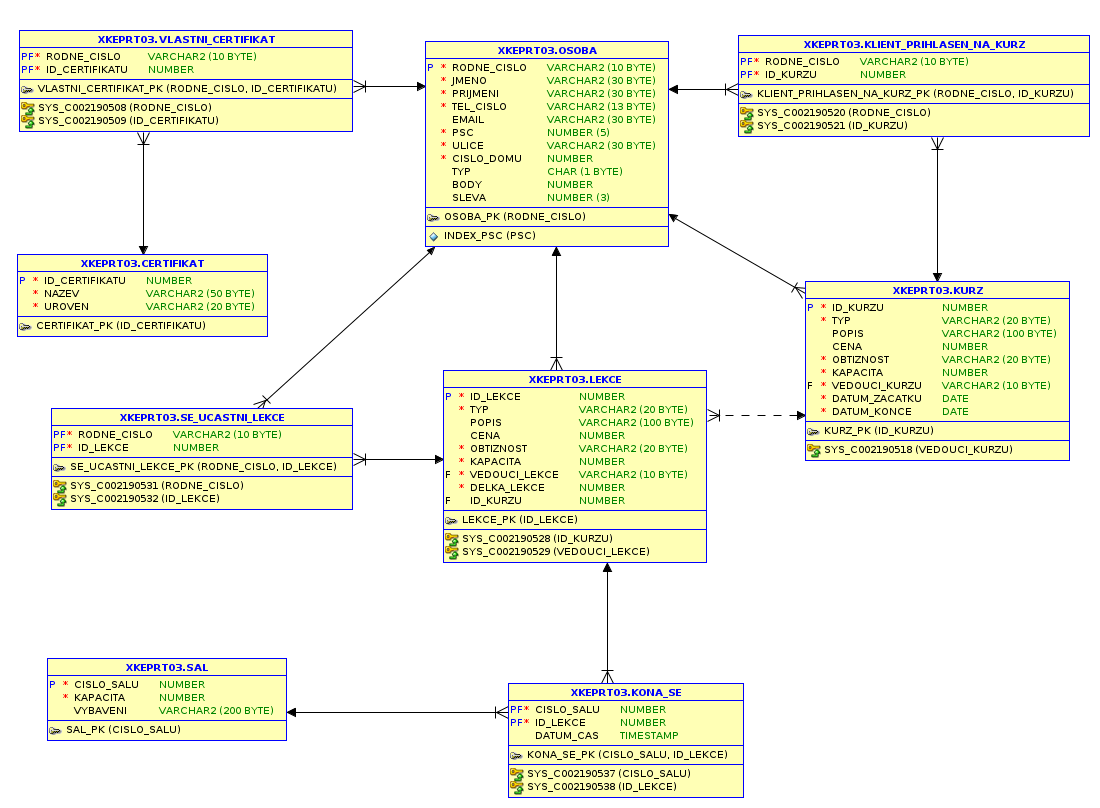
\includegraphics[scale=.538]{schema_DB.png}    
    \label{lopata}
\end{figure}
\restoregeometry

\section{Generalizácia}
V našej databáze je generalizácia reprezentovaná typom v entitnej množine osoba.
Typ predstavuje klienta symbolizovaného za pomoci znaku 'K' alebo inštruktora , ktorý je symbolizovaný
znakom 'I'. 

\section{Triggery}
Zadanie požadovalo implementovať trigger na generovanie hodnôt primárneho kľúča.
Trigger \texttt{ID\_lekce\_insert} generuje hodnoty primárneho kľúča tabuľky lekcie.

Nasledujúci trigger mal za úlohu kontrolovať vlastníctvo certifikátu osobou typu inštruktor a nápodobne bolo
treba kontrolovať, že kurz alebo lekcia je vedená osobou typu inštruktor. Pokial osoba
nieje inštruktor, trigger zahlási výnimku. 

Bol implementovaný trigger na kontrolu rodného čisla \texttt{kontrola\_rc}, podľa štandartných kritérii Českej Spávy Sociálního 
Zabezpečení. Pokiaľ je vložené neplatné rodné číslo, trigger zahlási výnimku. 

\section{Procedúry}
Vytvorili sme procedúru \texttt{prihlasit\_na\_kurz} aby osoba, ktorá sa prihlási na kurz bola automaticky
prihlásena aj na lekcie prislúhajúcemu kurzu. Procedúra využíva kurzor, ktorý vyhledá všetky lekcie daného kurzu.
Najprv je osoba prihlásená na kurz, potom sa prechádza kurzor a prihlasuje sa na jednotlivé lekcie. Pokial je osoba
prihlásená na lekciu pokračuje sa ďalej.

Taktiež bolo treba procedúru \texttt{odhlasit\_z\_kurzu}, ktorá zabezpečí 
aby osoba odhlasujúca z kurzu bola odhlásena aj zo všetkých lekcii daného kurzu. 

Procedúra \texttt{zmena\_vedouciho\_kurzu} zaistí zmenu vedúceho kurzu. Pokud procedúra prijme parameter 'Y'
tak zmena vedúceho nastane taktiež v lekciach, ktoré viedol starý vedúci kurzu.

\section{Explain plan}
Za pomoci príkazu explain plan sme boli schopný ukázať optimalizáciu spracovania dotazu za pomoci indexu.
Pri provom použití bola demonštrovaná verzia bez indexu čo ma malo za následok prechádzanie celej tabulky.
Nasledovalo druhé použite explain plan kde spracovanie toho istého dotazu bolo obohatené o optimalizáciu.
Namiesto prechádzania tabulky sa využilo prechádzanie  indexov čo sa značne prejavilo na cene operácii.

\section{Práva}
Na pridelenie práv členovi tímu boli použíte príkazy grant all on a grant execute on.
Grant all on udeľuje práva na prácu s tabulkami a grant execute on udeľuje práva na pracu s procedúrami.
\end{document}
